\documentclass[10pt,a4paper]{article}
\usepackage[utf8]{inputenc}
\usepackage[english]{babel}
\usepackage[T1]{fontenc}
\usepackage{amsmath}
\usepackage{amsfonts}
\usepackage{amssymb}
\usepackage{makeidx}
\usepackage{graphicx}
\usepackage{fourier}
\usepackage{listings}
\usepackage{color}
\usepackage[left=2cm,right=2cm,top=2cm,bottom=2cm]{geometry}
\author{Johannes Scheller, Vincent Noculak Lukas Powalla}
\title{Computational Physics - Project 1}
\begin{document}
\lstset{language=C++,
	keywordstyle=\bfseries\color{blue},
	commentstyle=\itshape\color{red},
	stringstyle=\color{green},
	identifierstyle=\bfseries,
	frame=single}
\maketitle
\newpage
\tableofcontents
\newpage
\section{Introduction to Project 1}
In physics, we often have to deal with differential equations o second order, which can be generally written in the from
\begin{equation}
	\frac{d^{2}y}{dx1{2}}+k^2(x)y=f(x)\quad,
\end{equation}
where we call $f$ the inhomgeneous term and $k^2(x)$ is a real function. A special case of these cases is Poisson's equation, which reads in the one-dimensional, spherical case
\begin{equation}
	\frac{1}{r^2}\frac{d}{dr}\left(r^2\frac{d\Phi}{dr}\right)=-4\pi\rho\left(\mathbf{r}\right)\quad.
\end{equation}
Doing some substitutions, we can write this in the following, more general form:
\begin{equation}
	\label{diff}
	-u''(x)=f(x)
\end{equation}
In this project, we try to solve eq.\eqref{diff} with the boundary conditions $u(0)=u(1)=0$. Therefore, we have to discretize $f$ and $u$. We approximate $u(x)$ as $v_i$, using a grid of $n$ gridpoints $x_i=i\cdot h$. Thus, $h=1/(n+1)$ is our steplength. We will also write $f_i=f(x_i)=f(hi)$.\\Approximating the second derivative of $u$, we get
\begin{equation}
	\label{num}
	-\frac{v_{i+1}+v_{i-1}-2v_i}{h^2}=f_i
\end{equation}
Our goal is to solve this equation \eqref{num}. Therefore, we will rewrite it as a set of linear equations in matrix form.

\subsection{Rewriting the equation in matrix-form}
Eq \eqref{num} can be written as a set of linear equations in matrix form. Therefore, we have to do the following steps:
\begin{align}
	-\frac{v_{i+1}+v_{i-1}-2v_i}{h^2}&=f_i\nonumber\\
	\label{vorform}-\left(v_{i+1}+v_{i-1}-2v_i\right)&=h^2\cdot f_i\\
\end{align}
Assuming we have an $n\times n$-matrix $\mathbf A$ of the following form

\begin{equation}
{\bf A} = \left(\begin{array}{cccccc}
2& -1& 0 &\dots   & \dots &0 \\
-1 & 2 & -1 &0 &\dots &\dots \\
0&-1 &2 & -1 & 0 & \dots \\\dots
& \dots   & \dots &\dots   &\dots & \dots \\
0&\dots   &\dots  &-1 &2& -1 \\
0&\dots    &\dots  & 0  &-1 & 2 \\
\end{array} \right)\quad,
\end{equation}
then we can rewrite this matrix in index notation as
\begin{equation}
\label{index}
	a_{ij}=\begin{cases}
		2&\mbox{if }i=j\\
		-1&\mbox{if  }|i-j|=1\\
		0&\mbox{else}
	\end{cases}\quad.
\end{equation}
Using this, we can also rewrite the multiplication $\mathbf{w}=\mathbf{A}\cdot\mathbf{v}$ with an $n$-dimensional vector $\mathbf v$ in the following way:
\begin{equation}
	w_i\quad\underset{\mathrm{def}}{=}\quad\sum_{j=1}^{n}a_{ij}\cdot v_j\quad\underset{\eqref{index}}{=}\quad -v_{i-1}+2v_i-v_{i+1}
\end{equation}
By using this result and substituting $h^2\cdot f_i\rightarrow\bar{b}$ in eq \eqref{vorform}, we get to the following equation:
\begin{equation}
	\mathbf{A \cdot v}=\bar{\mathbf{b}}
\end{equation}
with matrix $\mathbf{A}$ as given above. This is a set of linear equations that we are going to solve with our programm. In this example, we will assume that $f(x)$ is given by $f(x)=100\mathrm{e}^{-10x}$. Thus, the analytical solution of eq \eqref{diff} is given by $u(x)=1-(1-\mathrm{e}^{-10})x-\mathrm{e}^{-10x}$. We will later compare our numerical results to this solution.

\section{Different algorithm to solve this set of linear equations}

In this chapter, We want to solve the given set of linear equations first by solving it with a self-programmed algorhithm. Furthermore, we want to compare the produced numerical solution to the exact solution and calculate the maximum relative error for a given number of Gridpoints. 
In order to know, whether our algorithm is best to solve this set of linear equations, we want to compare this algorhith with LU-decomposition and Gaussian algorhitm with respect to the floating point operations and the calculation time. 

\subsection{self-programmed algorithm }

As we have shown in the previous capture, you can rewrite the set of linear equations as product of a matrix and a vector:
\begin{equation}
	\mathbf{A \cdot v}=\bar{\mathbf{b}}
\end{equation}
In this case, the matrix A is a tridiagonal matrix. This means, that it is possible to interpret this matrix as 3 vectors because all other components of the matrix are zero and will stay zero. This gives us the advantage that we don't have to deal with 2-dimensional Arrays and we can dump the number of floating operations (compared to LU-decomposition/Gaussian-algorithm)

The programmed algorithm will work in the following way. First, we want to reach a upper diagonal matrix by vector-additions/subtractions. Second, We want to bring the matrix to a diagonal form and at last, we scale the solution vector. The first two steps also effekt the solutionvector (in our case btilde[] ). We programmed following souce-code (extract):

extract of the used algorithm((12 floating operations):
\begin{lstlisting}
//first
for(int i=0;i<n+1;i++){
	b[i+1]=b[i+1]-c[i]*(a[i+1]/b[i]);
	btilde[i+1]+=-(a[i+1]/b[i])*btilde[i];
}
//second
for(int i=n;i>0;i--){
	btilde[i-1]+=-btilde[i]*(c[i-1]/b[i]);
}
//normalization
for(int i=0;i<n+1;i++){
	btilde[i]=btilde[i]/b[i];
}
\end{lstlisting}
	
	
As you can see, we use at the moment 12n floating point operations for the mainalgorithm. If we look closer at the algorithm, we will see that you can simplify a lot by skipping unnecessary arithmetic operations. 
We managed to get to 6 Floating point operations:
\begin{lstlisting}
//first
for(int i=0;i<n+1;i++){
	b[i+1]=b[i+1]-1/b[i];
	btilde[i+1]=btilde[i+1]+btilde[i]/b[i];
}
//second and normalization
for(int i=n;i>0;i--){
	btilde[i-1]=(btilde[i-1]+btilde[i])/b[i];	
}
\end{lstlisting}
	
\subsection{Gaussian elimination}


\subsection{LU-decomposition}

In the LU-decompsition we factorize the matrix $\mathbf A$ as the product of a lower($\mathbf L$) and an upper($\mathbf{U}$) triangular matrix. As a consequence we get the following equation:

\begin{equation}
\mathbf{L \cdot U \cdot v = \bar{b}}
\end{equation}

If we say $\mathbf{U \cdot v = w}$, we get two systems of linear equations which need to be solved.

\begin{gather}
\mathbf{L \cdot w = \bar{b}} \\
\mathbf{U \cdot v = w}
\end{gather}

While solving (14) and (15) only need $\sigma(n^2)$ flops, which is less compared to the gaussian elimination, factorising $\mathbf{A}$ as in (12) takes $\sigma(n^3)$ flops. In total the LU-decomposition does take to the power of two flops more than our algorithm. In our project it takes more flops than the gaussian elimination too.


\section{Resuluts and discussion of the self-programmed algorithm}

We solved the linear set of equation with a different number of Gridpoints. This means, that we discretise the used funktions and approximated them with n Gridpoints. If you take a closer look at the given solutions produced with our algorithm, you will notice that the numerical approximation seems to converge to the exact solution. (for n=10...$10^5$) In the figure \ref{Comparison10}, you can see the numerical solution for 10 Gridpoints. The numerical approximation doesn't fit very well with the exact solution, however the boundary conditions seem to be fullfilled. We run our programm with diferend numer of Gridpoints. The figure with 100 Gridpoints you can find in figure \ref{Comparison100}, the figure with 1000 Gridpoints you can find in \ref{Comparison1000} and the figure with $10^5$ Gridpoints you can find in figure \ref{Comparison100000}. 


\begin{figure}[h]
\centering
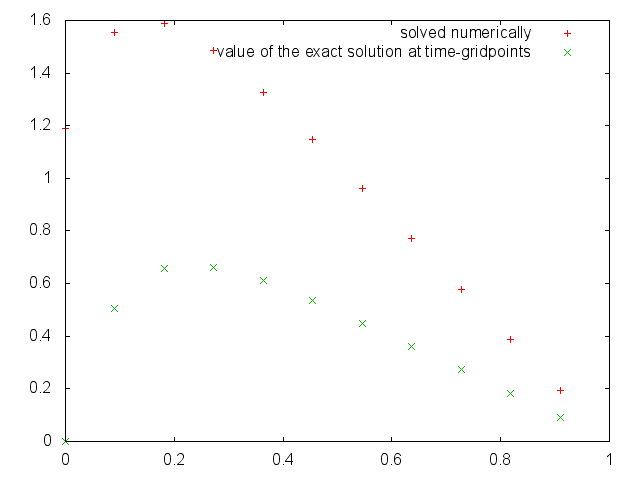
\includegraphics[scale=0.5]{Comparisonplot10.png}
\caption{Plot of the exact solution and the numerical solution for 10 Gridpoints}
\label{Comparison10}
\end{figure}

\begin{figure}[h]
\centering
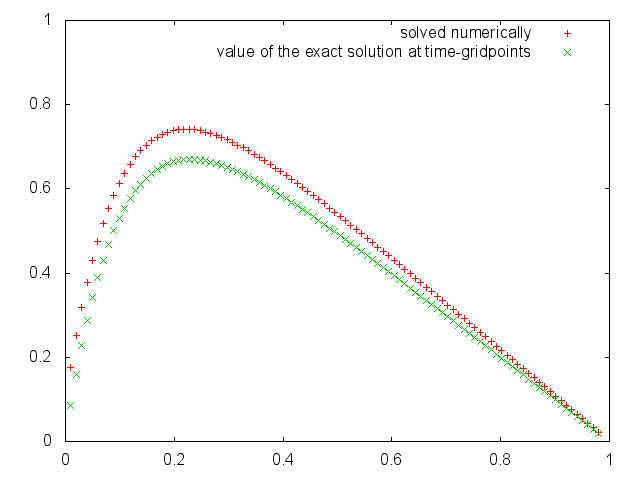
\includegraphics[scale=0.5]{Comparisonplot100.png}
\caption{Plot of the exact solution and the numerical solution for 100 Gridpoints}
\label{Comparison100}
\end{figure}

\begin{figure}[h]
\centering
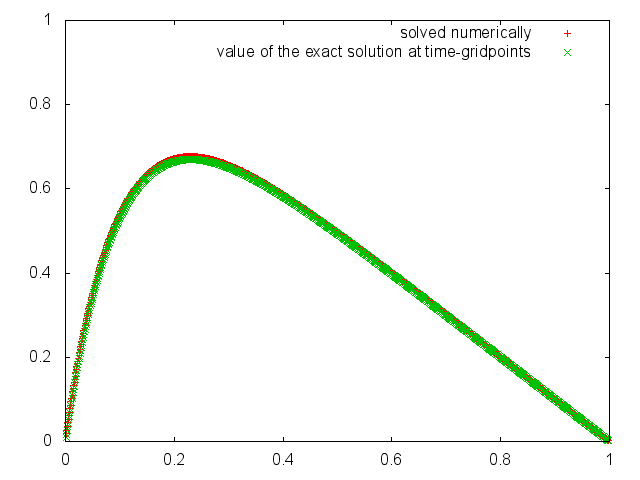
\includegraphics[scale=0.5]{Comparisonplot1000.png}
\caption{Plot of the exact solution and the numerical solution for 1000 Gridpoints}
\label{Comparison1000}
\end{figure}

\begin{figure}[h]
\centering
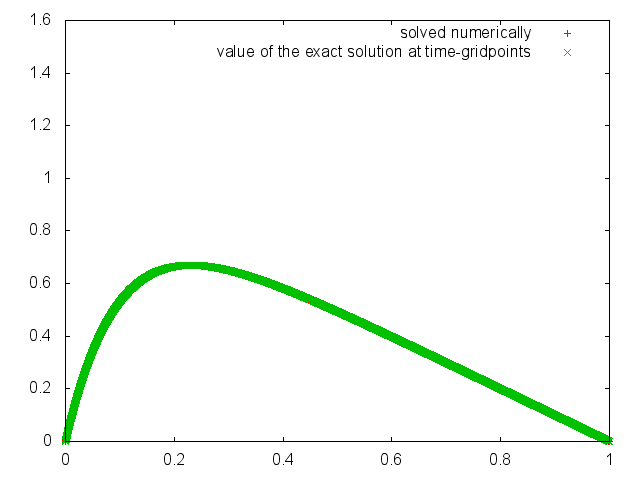
\includegraphics[scale=0.5]{Comparisonplot100000.png}
\caption{Plot of the exact solution and the numerical solution for 100000 Gridpoints}
\label{Comparison100000}
\end{figure}

In the next step, we want to compare our results with exact solution. Therefore, we estimated the relative error for different step length. 

\begin{figure}[h]
\centering
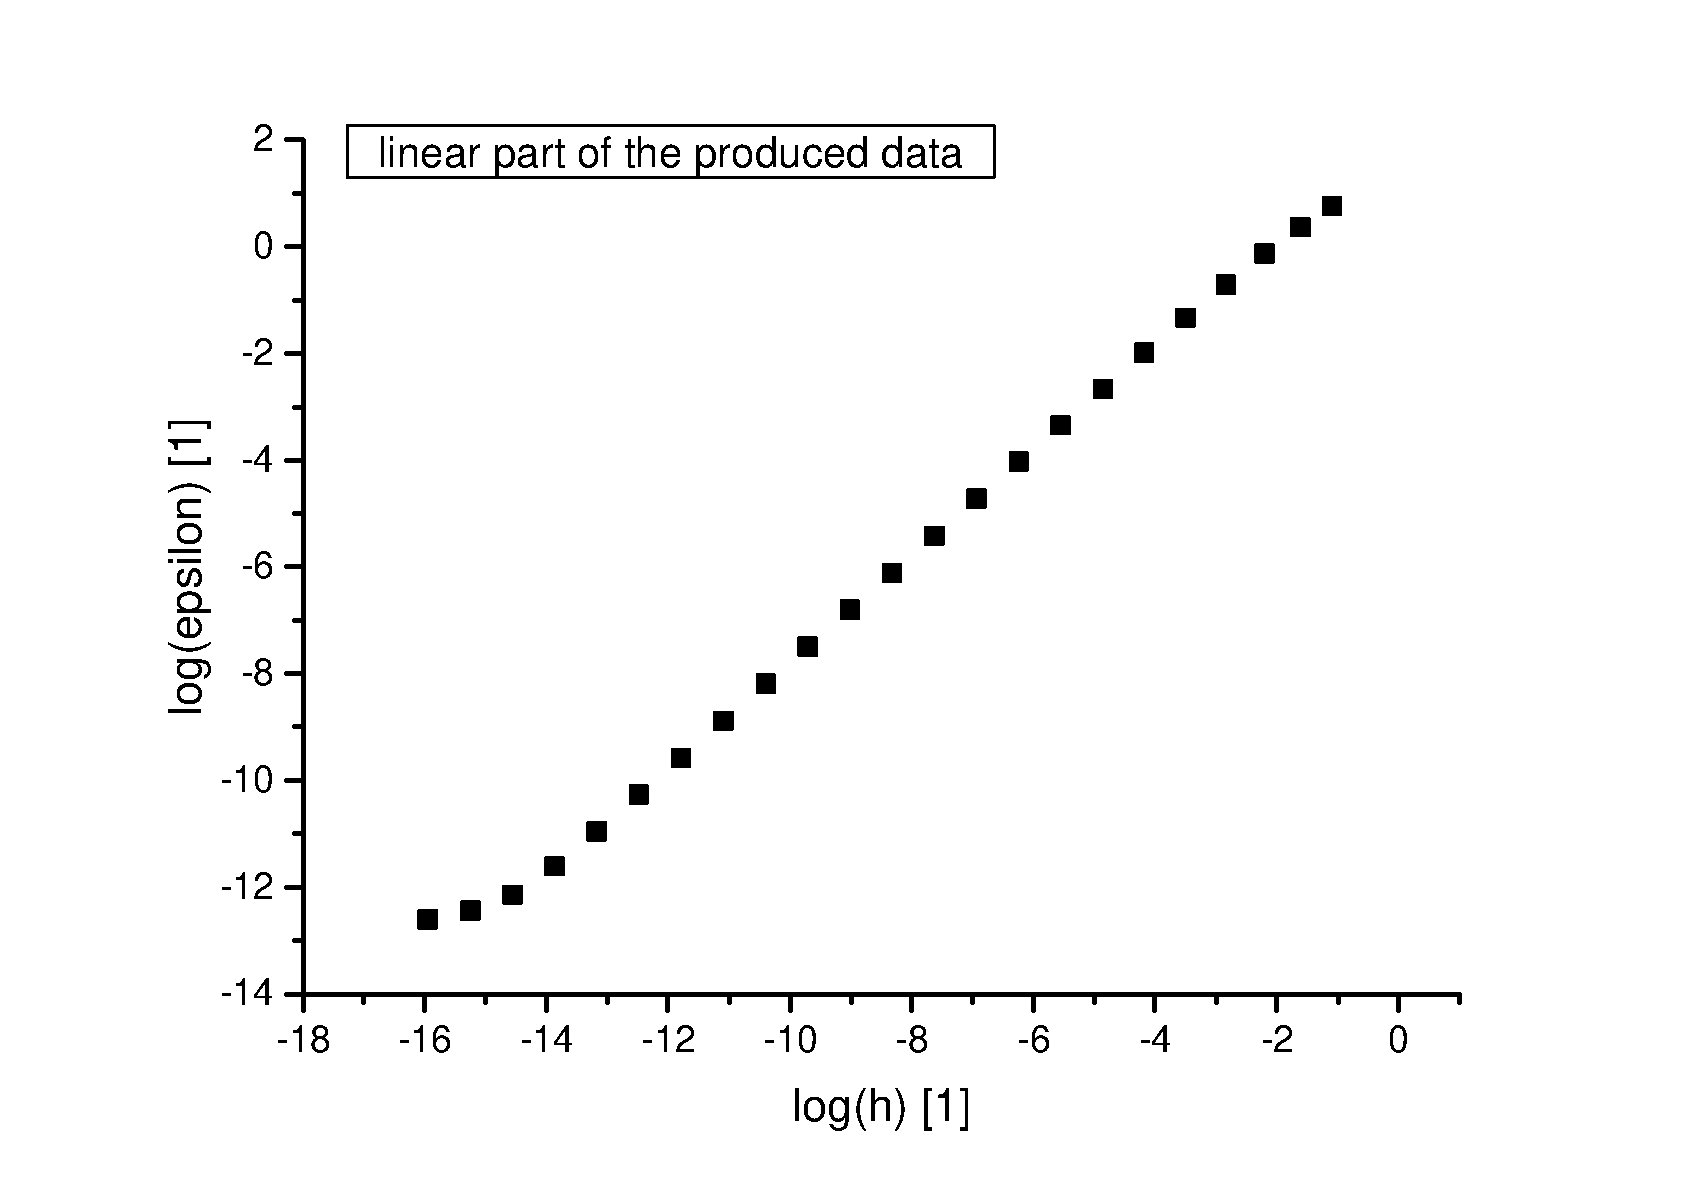
\includegraphics[scale=0.5]{epsilon_plot_log.pdf}
\caption{The epsilon is the maximum of the Epsilonerror for given Number of Gridpoints n (and Steplenght h) }
\label{linear plot}
\end{figure}

\section{Comparison of self-programmed algorithm, Gaussian elemination and LU Decomposition }




\end{document}